\chapter{Deep Learning for Images}

{\sf Let's imagine we have a fully connected network for image recognision and the problem is the bigger network we get the more connections the network has (more prompt of overfitting the network has, more computing pover needs for trainig). The main idea of deep learning is imposing a structure on that network. Rather than have a fully connected network we can have a structured network with less number of weights but more effective for solving specific task.}

\section{Convolution}

Deep leaning was enspired by biology. In the early 1950's professors David Hubel and Torsten Wiesel made \href{https://youtu.be/IOHayh06LJ4}{series of experiments} on cat's brain. They tried to answer how cats see the world around them, how their visual cortex works. The experiments were putting a cat in some locking mechanism, closing one eye of the cat that only annoys input from one eye. Then they drill a little hole in it's head and put an electrode at different place of the visual cortex to see how specific neurons reacts to specific visual stimulus. The cat saw some lines. So they found that some neuron best detects lines with one angle, while some others detects lines with another angle [\href{https://www.ncbi.nlm.nih.gov/pmc/articles/PMC1363130/pdf/jphysiol01298-0128.pdf}{ссылка} на статью для интересующихся].

\subsubsection*{Detecting lines}

So if a cat sees with lines let's ask neural network to see with lines. The detection of lines at various shapes was already known at that point and it was done in convolutions. The convolution is just pointwise multiplication and then addition it. You can see [pic. 7.1] the green tensor what is our input image, the yellow part of it is convolution filter and the red numbers are the values of this filter. What we do is we multiply each pixel value at red number and then we sum them up.\\
\begin{figure}[h]
  \centering
  \begin{tabular}{cccc}
    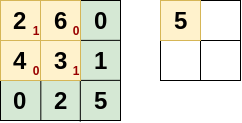
\includegraphics[width=0.2\linewidth]{7a.png} &
    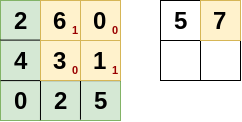
\includegraphics[width=0.2\linewidth]{7b.png} &
    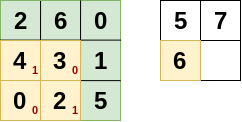
\includegraphics[width=0.2\linewidth]{7c.png} &
    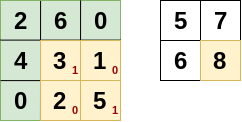
\includegraphics[width=0.2\linewidth]{7d.png} \\
    $2\cdot1+3\cdot1=5$ & $6\cdot1+1\cdot1=7$ & $4\cdot1+2\cdot1=6$ & $3\cdot1+5\cdot1=8$ \\
    & & & \\
    \multicolumn{4}{c}{(7.1) Convolution filter}
  \end{tabular}
\end{figure}
[В примере выше изображение было черно-белым: оно состояло из одного канала. Если же каналов больше, например, 3, то наш фильтр будет состоять уже из 3 слоев, необязательно одинаковых. Однако после прохода таким фильтром у изображения все равно останется один канал. Далее при указании размера фильтра я буду указывать размер одного слоя.]\\
So the parameters what we are trying to optimise are kernels (size of the filter) and strides (how large shift of the filter we use). You can see here [pic. 7.2] how various convolutions detect various feature of the image:\\
\begin{figure}[h]
  \centering
  \begin{tabular}{ccc}
    $ \begin{pmatrix}
      0 & 0 & 0 \\
      0 & 1 & 0 \\
      0 & 0 & 0 \\
    \end{pmatrix} $ &
    $ \begin{pmatrix}
      1 & 0 & -1 \\
      0 & 0 & 0 \\
      -1 & 0 & 1 \\
    \end{pmatrix} $ &
    $ \begin{pmatrix}
      -1 & -1 & -1 \\
      -1 & 8 & -1 \\
      -1 & -1 & -1 \\
    \end{pmatrix} $ \\
    & & \\
    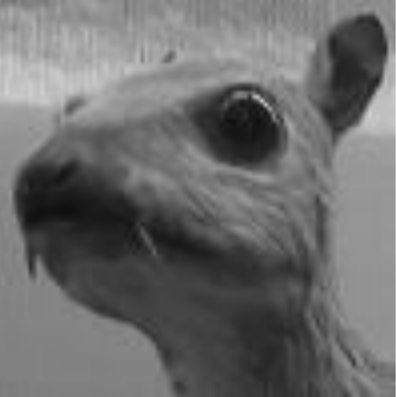
\includegraphics[width=0.2\linewidth]{7e.png} &
    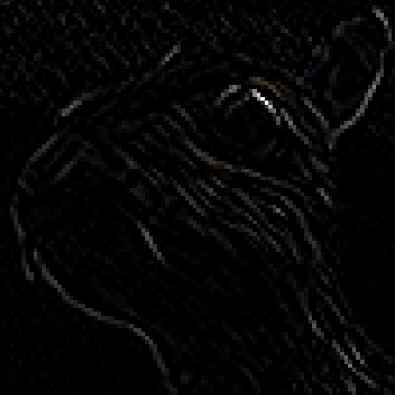
\includegraphics[width=0.2\linewidth]{7f.png} &
    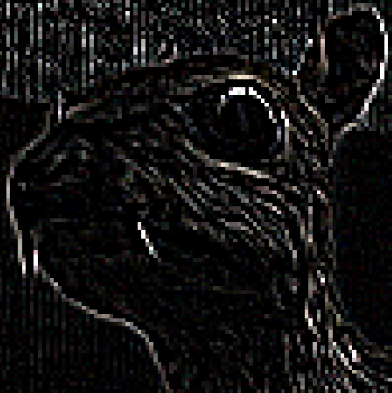
\includegraphics[width=0.2\linewidth]{7g.png} \\
    & & \\
    \multicolumn{3}{c}{(7.2) After applying some convolutions}
  \end{tabular}
\end{figure}

\subsubsection*{Convolution layers}

If you have simple shapes detecting then you can have the more complex shapes detecting. You can get that complex shapes detecting by applying convolution to the features you get after you apply convolution first time. And so on. So now we have a several convolution levels. What is important to understand that there is still neurons, there is still multiplication of preceptron input by weight. So all the math is still the same. When we back propagate the gradient we just sum not over all neurons but over specific neurons because all neurons in one convolution layer have the same weight.\\
Now let's imagine you have a typical image with size $224\times224\times3$ (3 because of color channels). It is called 2D convolution because it doesn't scan in depth. The next step is going over all image and take values what your filters outputs. And you have several different convolutions (every convolution has it's own filter). And what you get when you go with convolution over all picture is your convolved feature (or convolution map or your feature map). That black image with white edges of a deer is a convolution map. So you have set of some different maps and the next convolution layer looks at each map of the set like color channels (so it's still 2D convolution).\\
\begin{figure}[h]
  \centering
  \begin{subfigure}[l]{0.6\linewidth}
    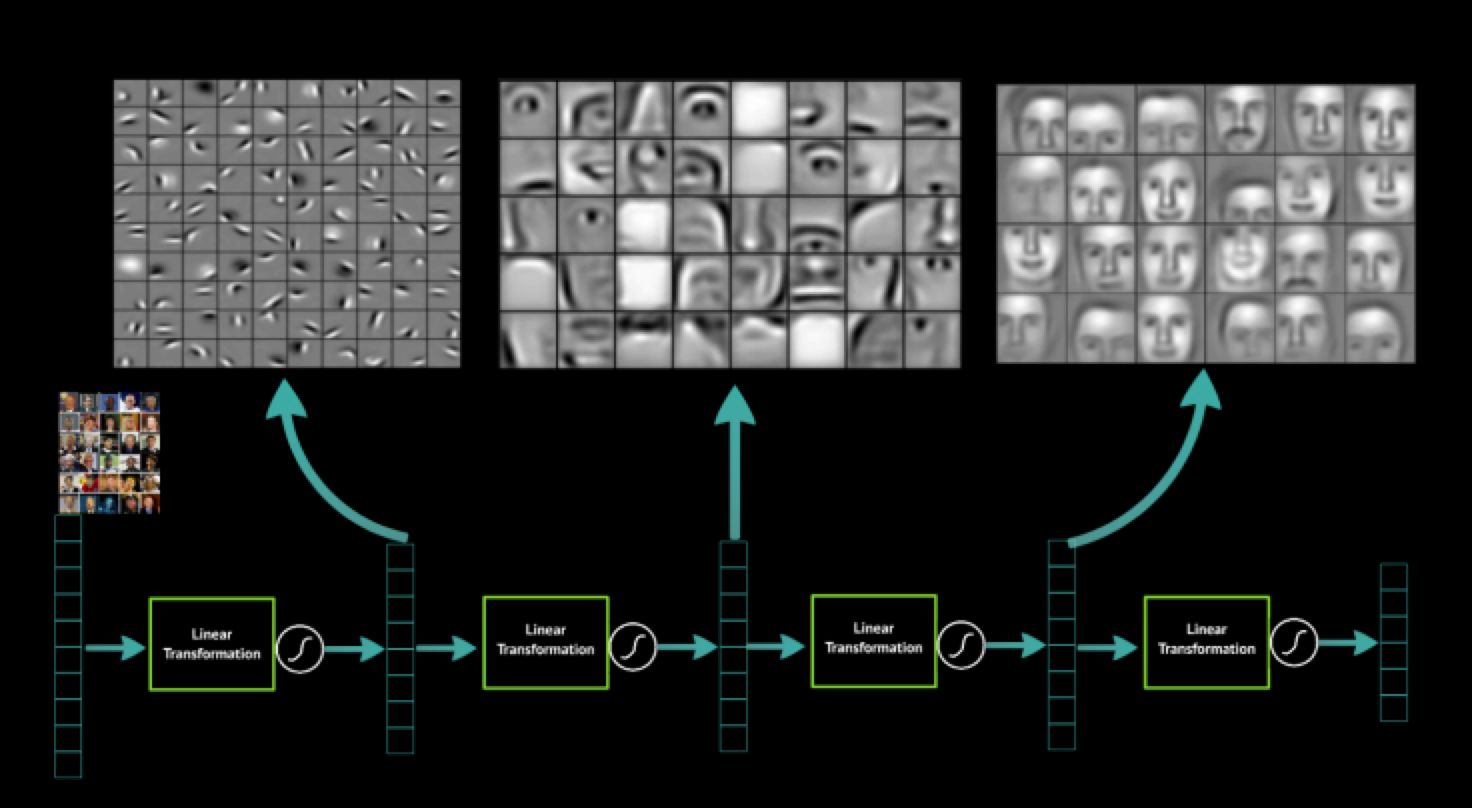
\includegraphics[width=\linewidth]{7h.png}
    \caption*{(7.3) Convolution layers}
  \end{subfigure}
\end{figure}

\vspace{-0.5cm}
\subsubsection*{Pooling}

The another operation what we use to decrease the complexity is called pooling. For example, if there is a clear signal on a some area of a feature map, then we just need a point with that signal because all the neightboring points probably are signaling the same. So we just take the maximum and it's called the maximum pooling. Also in some cases you can take average (and you'll have the average pooling).

\subsubsection*{Padding}

Padding is one way to perform convolution. For example, we have an image of size $M\times N$ and a filter of size $(2K+1)\times(2K+1)$. Before start moving the filter, we resize the original image to $(2K+M)\times(2K+N)$, adding a frame with weight $K$, consisting of zeros.

\section{Examples of Deep Neural Networks}
\vspace{-0.6cm}
\subsubsection*{LeNet-5}

The one of the first deep learning network. It was created in 1998 and it use all the algorithms and computer vision technics of that time. Also it used only 61470 weights. After that network there was a deep learning winter: almost noone works with them (except the several labs across the world) until 2012.

\subsubsection*{AlexNet}

In 2012 there was a ImageNet competition when AlexNet won by a huge margin with 15\% error (the result in 2011 were like 1st place had 27\%). This is the first deep network that proved to be so much ahead of everything else, and after that people start do all with deep learning.
AlexNet is a deep neural network what has 100,207,632 weights and it uses a GPU's calculations (what made this net successful in 2012). Also it has two parts each calculated individually on its own GPU. So there are some features of this net:\\
\begin{enumerate}[label=$\bullet$]
  \item Scales all images to $256\times256$, then takes random $224\times224$ batches and mirrors them.
  \item Substracts average pixel value from each pixel.
  \item ReLU ($\max(0,x)$).
  \item Dropout 0.5.
  \item Batch size 128, SGD with momentum 0.9 (momentum is how much of the previous gradient descent steps you keeps), L2 weight decay ($\lambda=0.0005$).
\end{enumerate}
The kernels on GPU 1 are largely color-agnostic, while the kernels on on GPU 2 are largely color-specific. This kind of specialization occurs during every run and is independent of any particular random weight initialization (modulo a renumbering of the GPUs) [\href{https://www.nvidia.cn/content/tesla/pdf/machine-learning/imagenet-classification-with-deep-convolutional-nn.pdf}{ссылка} на статью с более подобным описание для интересующихся].\\
Today we don't use the AlexNet, we use one of three things: VGGNet, Inception network or ResNet.

\subsubsection*{VGGNet}

VGGNet is a very deep convolutional network (VGG is the lab what invented it). The main idea is replace some layers of wide convolutions by more layers of $3\times3$ convolutions. It works because several layers of $3\times3$ have less weights than a big initial convolution. So it saves weights and it's very deep (but not heavy computantionaly). VGGNet is still used today in case of missing Google resources.

\subsubsection*{Inception network}

But is we have Google resources we can do something more complex. There are two main ideas of Inception network (it is named after the self-titled movie). The first is using $1\times1$, $3\times3$ and $5\times5$ convolutions in one layer and then concatenating the results. The second idea is to use $1\times1$ convolutions to made other filters flat. So there are inception modules:\\
\begin{figure}[h]
  \centering
  \begin{subfigure}[l]{0.4\linewidth}
    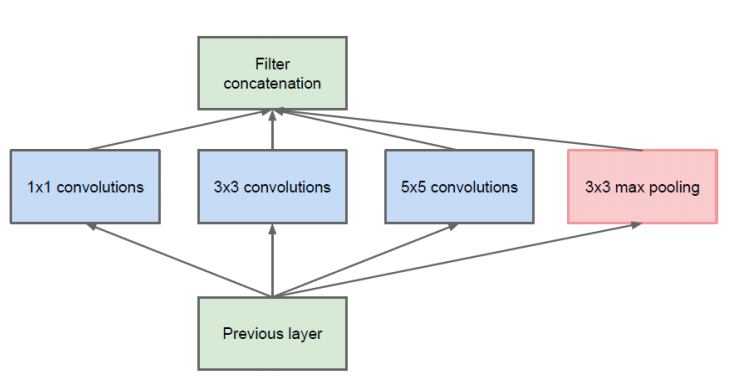
\includegraphics[width=\linewidth]{7i.png}
  \end{subfigure}
  \hspace{0.5cm}
  \begin{subfigure}[r]{0.4\linewidth}
    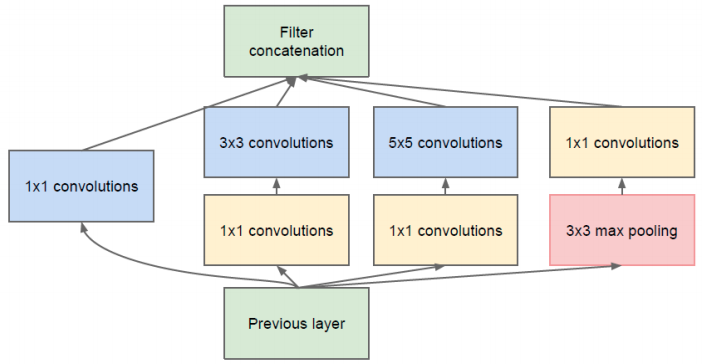
\includegraphics[width=\linewidth]{7j.png}
  \end{subfigure}
  \caption*{(7.4) Inception modules}
\end{figure}
And there are Inception network (also it named GoogLeNet):
\begin{figure}[h]
  \centering
  \begin{subfigure}[c]{0.7\linewidth}
    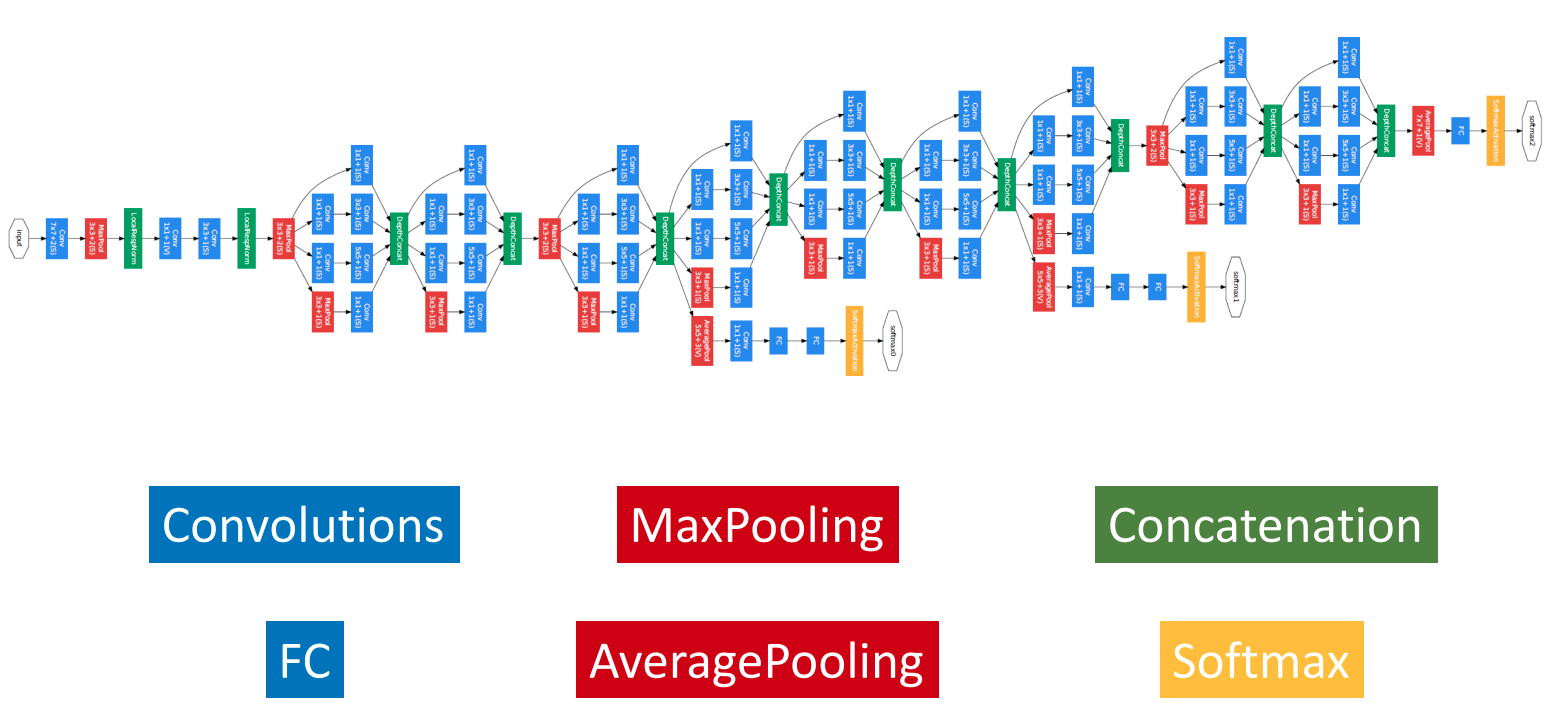
\includegraphics[width=\linewidth]{7k.png}
    \caption*{(7.5) GoogLeNet}
  \end{subfigure}
\end{figure}

\vspace{-0.5cm}
\subsubsection*{ResNet}

As you can see the GoogLeNet has multiple outputs. The reason is the information is lost the deeper you go --- it is nice to have an information from the different layers. But instead of it we can do additional information: add the output from the previous layer to the output of next layer. It is called a residual connection [pic. 7.6] (also called skip connections). Also we have a highway connection [pic. 7.7]: when you train in a separate neural network to determine how much of the output we add and how much of the previous input we keep.\\
\begin{figure}[h]
  \centering
  \begin{subfigure}[l]{0.31\linewidth}
    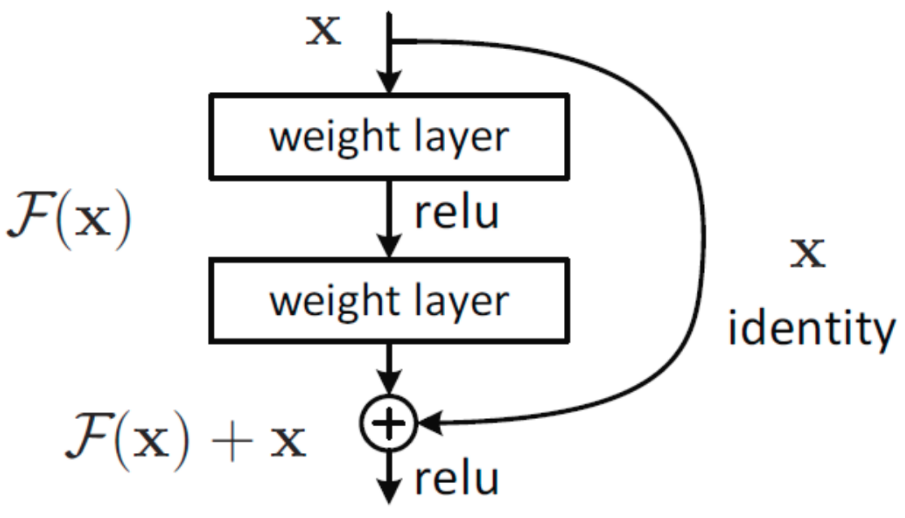
\includegraphics[width=\linewidth]{7l.png}
    \caption*{(7.6) Residual connection}
  \end{subfigure}
  \hspace{2cm}
  \begin{subfigure}[r]{0.4\linewidth}
    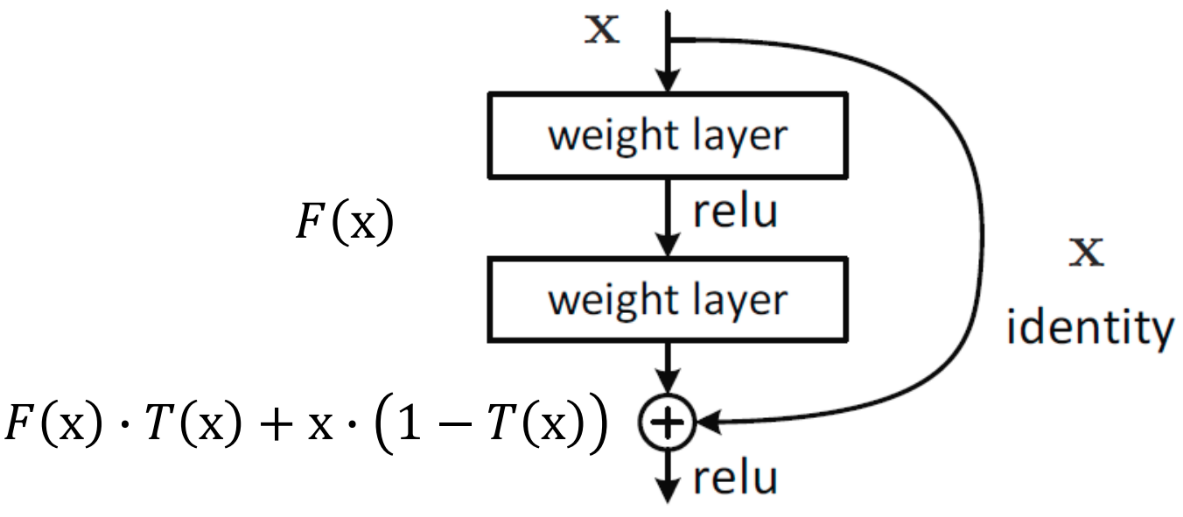
\includegraphics[width=\linewidth]{7m.png}
    \caption*{(7.7) Highway connection}
  \end{subfigure}
\end{figure}
So this ideas used in ResNet. ResNet is the widely used deep learning network. It has error rate only 3.57\%. However, if you want have less weights, you'll go to VGG: it still works well (now it has error rate 6.8\%).\\
The problem of that error rate is that human error rate is near 5\%. And error rate less than 5\% means the training on noice because all image dataset created by humans. So after the 2015 image networks changed from image classification to object detection.

\section{Technics in Image Analysis}
\vspace{-0.6cm}
\subsubsection*{Image augmentation}

The data is almost never enough. There is some ways to make your dataset bigger:\\
\begin{enumerate}[label=$\bullet$]
  \item Flip image. Be carefull, some flipped objects can be from another class: car upside down in come cases may be a trash.
  \item Rotate image. When you rotate, for example, on 45 degrees you may interpolate the result: fill the corners using a part of initial picture [pic. 7.8] or using the edge pixels of rotated image [pic. 7.9].\\
  \begin{figure}[h]
  \centering
  \begin{subfigure}[l]{0.2\linewidth}
    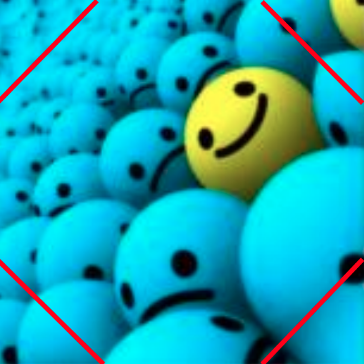
\includegraphics[width=\linewidth]{7o.png}
    \caption*{(7.8) Symmetric}
  \end{subfigure}
  \hspace{2cm}
  \begin{subfigure}[r]{0.2\linewidth}
    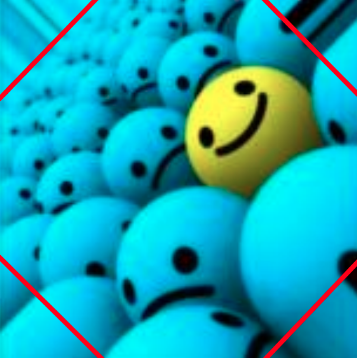
\includegraphics[width=\linewidth]{7n.png}
    \caption*{(7.9) Edge}
  \end{subfigure}
\end{figure}
  \item Crop image. This is very powerfull because it can get a lot of images.
  \item Scale image.
  \item Use Gaussian noice. After using a noice it becomes harder to overfit.
  \item Shift the colors by some constant. Good method of color shifting is transfering at the other color space and shiffting after that.
\end{enumerate}

\subsubsection*{Transfer Learning and Finetuning}

If image augmentation doesn't work, you have a transfer leaning. It is the most imprortant technic you can use on the image analysis. For example, someone has trained on ResNet and published all of it. The weights of his neural net is just a calculation of some image features. It doesn't matter what featers they are: dogs, cars etc; you can train on them. So the fransfer learning is training deep network on a big dataset, for example, ImageNet, then taking the result of that calculations as features, freeze it and training your small part for your specific task on output of the frozen part. It works wonderfully for any task, because there are so many features in the frozen part.\\
If you have many data you can use finetuning. The finetuning is like transfer learning but you don't fix other network weights. And you still train (finetune) to your task. Sometimes it helps but almost over it is overfitting becase the fisrt part is designed for millions and millions of images.